% Volume I — Physical electromagnetic figure library (FINAL illustration pass)
% Classical line drawings: geometry, fields, sources, surfaces — no workflow boxes.

\usetikzlibrary{decorations.pathmorphing,patterns,patterns.meta}

\tikzset{
  voliphys/.style={
    every node/.style={font=\footnotesize, text=black},
    line cap=round,
    line join=round,
    scale=1.0
  },
  voliaxis/.style={-{Latex[length=2mm,width=1.4mm]}, line width=0.7pt, black},
  volishell/.style={line width=0.75pt, draw=black},
  volishelld/.style={line width=0.65pt, dashed, draw=black},
  volisrc/.style={fill=black, circle, inner sep=1.6pt},
  volifield/.style={-{Latex[length=1.8mm,width=1.2mm]}, line width=0.55pt, black},
  volipoynt/.style={-{Latex[length=1.8mm,width=1.2mm]}, line width=0.55pt, black},
  volilabel/.style={font=\footnotesize, inner sep=1pt, fill=white, fill opacity=0.96, text=black},
  volihatch/.style={pattern=north east lines, pattern color=black!40}
}

% --- Fig. 1.2: source, enclosing surface, angular representation ---
\newcommand{\VolIPhysThreeLevelHierarchy}{%
\begin{tikzpicture}[voliphys]
  \coordinate (O) at (0,0);
  \draw[volishell, fill=black!5] (O) circle (0.55);
  \node[volilabel] at (0,-0.85) {$\Omega_s$};
  \draw[volifield] (0.12,0.08) -- ++(0.38,0.14) node[right,font=\scriptsize] {$\Jimp$};
  \draw[volishell] (O) circle (1.35);
  \node[volilabel] at (1.55,0.35) {$\Gamma_R$};
  \draw[volifield] (1.05,0.28) -- ++(0.42,0.12) node[right,font=\scriptsize] {$\E$};
  \draw[volipoynt] (1.05,-0.28) -- ++(0.38,-0.18) node[right,font=\scriptsize] {$\H$};
  \draw[volipoynt] (0.95,0.95) -- ++(0.25,0.35) node[above,font=\scriptsize] {$\hat{\mathbf{n}}$};
  \node[volilabel, align=center] at (0,1.65) {$(\E,\H)$ on $\Gamma_R$};
  \draw[volishell] (O) circle (2.15);
  \foreach \a in {25,65,115,155,205,245,295,335} {
    \draw[volifield] (\a:1.72) arc [start angle=\a, end angle=\a+28, radius=1.72];
  }
  \node[volilabel, align=center] at (0,-2.45) {$\E_t(\theta,\phi)$ on $S^2$};
\end{tikzpicture}%
}

% --- Ch.1 Fig. 1.3: matched impressed source vs rim template on same aperture ---
\newcommand{\VolIPhysMatchedAperture}{%
\begin{tikzpicture}[voliphys]
  \begin{scope}
    \draw[volishell, fill=black!5] (0,0) circle (0.72);
    \node[volilabel] at (0,-1.05) {aperture radius $a$};
    \draw[volifield] (-0.32,-0.05) -- (0.22,0.14) node[midway,above,font=\scriptsize] {$\Jimp$};
    \draw[volishell] (0,0) circle (1.38);
    \node[volilabel, font=\scriptsize] at (1.05,0.55) {$\Gamma_R$};
    \foreach \a in {25,70,115,205,250,295} {
      \draw[volipoynt] (\a:1.08) -- (\a:1.28);
    }
    \node[volilabel, align=center, font=\scriptsize] at (0,1.55) {Maxwell-consistent\\impressed current};
  \end{scope}
  \begin{scope}[shift={(3.35,0)}]
    \draw[volishell, fill=black!5] (0,0) circle (0.72);
    \draw[volishelld, line width=0.9pt, gray!50!black] (0.72,0.1) arc (10:170:0.72);
    \node[volilabel, font=\scriptsize, gray!50!black] at (0,0.28) {$\E_t$};
    \node[volilabel, font=\scriptsize] at (0,-0.32) {prescribed only};
    \draw[volishell] (0,0) circle (1.38);
    \node[volilabel, font=\scriptsize] at (1.05,0.55) {$\Gamma_R$};
    \foreach \a in {25,70,115,205,250,295} {
      \draw[volipoynt, opacity=0.35] (\a:1.08) -- (\a:1.28);
    }
    \node[volilabel, align=center, font=\scriptsize] at (0,1.55) {tangential template\\without matching $\Jimp$};
  \end{scope}
\end{tikzpicture}%
}

% --- Fig. 1.5: vacuum constitutive link (physical vectors) ---
\newcommand{\VolIPhysVacuumClosureMap}{%
\begin{tikzpicture}[voliphys]
  \draw[voliaxis] (-1.8,0) -- (1.8,0) node[right, font=\scriptsize] {$\mathbf{k}$};
  \draw[volifield] (-1.2,0) -- (-1.2,0.75) node[above, font=\scriptsize] {$\E$};
  \draw[volifield] (-0.55,0) -- (-0.55,0.75) node[above, font=\scriptsize] {$\H$};
  \draw[volipoynt] (0.15,0) -- (0.15,0.65) node[above, font=\scriptsize] {$\D$};
  \draw[volipoynt] (0.75,0) -- (0.75,0.65) node[above, font=\scriptsize] {$\B$};
  \node[volilabel, font=\scriptsize] at (-1.2,-0.45) {$\D=\varepsilon_0\E$};
  \node[volilabel, font=\scriptsize] at (-0.55,-0.45) {$\B=\mu_0\H$};
  \node[volilabel, font=\scriptsize] at (1.35,0.35) {$\eta_0=\sqrt{\mu_0/\varepsilon_0}$};
\end{tikzpicture}%
}

% --- Source on finite support + observation sphere (Ch.2 spine, Ch.3.1) ---
\newcommand{\VolIPhysSourceObservationSphere}{%
\begin{tikzpicture}[voliphys]
  \draw[volishell, fill=black!4] (-0.35,-0.25) rectangle (0.35,0.25);
  \node[volilabel] at (0,-0.55) {$\operatorname{supp}\Jimp$};
  \draw[volishelld] (0,0) circle (1.05);
  \node[volilabel, font=\scriptsize] at (0.75,0.75) {reactive};
  \draw[volishell] (0,0) circle (1.85);
  \node[volilabel] at (0,2.05) {$\Gamma_R$};
  \foreach \a in {30,75,120,210,255,300} {
    \draw[volipoynt] (\a:1.55) -- (\a:1.78);
  }
\end{tikzpicture}%
}

% --- Maxwell solution then outgoing selection (Fig. 2.2) ---
\newcommand{\VolIPhysSourceRadiationSequence}{%
\begin{tikzpicture}[voliphys]
  \draw[volishell, fill=black!4] (-0.3,-0.2) rectangle (0.3,0.2);
  \draw[volifield] (0.35,0) -- (0.95,0.15) node[midway,above,font=\scriptsize] {$\mathcal{S}_\omega$};
  \draw[volishelld] (1.15,0) circle (0.55);
  \node[volilabel, font=\scriptsize] at (1.15,0.75) {full $(\E,\H)$};
  \draw[volipoynt] (1.75,0.05) -- (2.35,0.05) node[midway,above,font=\scriptsize] {$P_{\mathrm{rad}}$};
  \draw[volishell] (2.75,0) circle (0.55);
  \foreach \a in {45,135,225,315} {\draw[volipoynt] (2.75,0) ++(\a:0.35) -- ++(\a:0.22);}
  \node[volilabel] at (2.75,-0.85) {$\mathcal{F}_{\mathrm{rad}}$};
\end{tikzpicture}%
}

% --- State on sphere vs harmonic chart (Fig. 3.2) ---
\newcommand{\VolIPhysStateRepresentation}{%
\begin{tikzpicture}[voliphys]
  \begin{scope}
    \draw[volishell] (0,0) circle (0.9);
    \draw[volifield] (-0.5,0.2) -- (0.2,0.35);
    \draw[volipoynt] (0.3,-0.15) -- (0.75,-0.35);
    \node[volilabel] at (0,-1.15) {$\mathcal{R}_\omega[\Jimp]$};
  \end{scope}
  \node[volilabel, font=\scriptsize] at (2.0,0) {$\mathcal{C}$ on $\mathcal{F}_{\mathrm{rad}}$};
  \begin{scope}[shift={(3.2,0)}]
    \draw[volishell] (0,0) circle (0.9);
    \foreach \a in {0,40,80,120,160,200,240,280,320} {
      \draw[volipoynt] (\a:0.55) -- (\a:0.85);
    }
    \node[volilabel] at (0,-1.15) {$\{c_{\ell m}^{(\sigma)}\}$};
  \end{scope}
\end{tikzpicture}%
}

% --- Radiative Hilbert space: modes on sphere (Fig. 3.16 area) ---
\newcommand{\VolIPhysRadiativeHilbertModes}{%
\begin{tikzpicture}[voliphys]
  \draw[volishell] (0,0) circle (1.2);
  \draw[volishelld] (0,0) circle (0.55);
  \draw[volishelld] (0,0) circle (0.85);
  \node[volilabel] at (0,1.45) {$\mathcal{F}_{\mathrm{rad}}$};
  \draw[volifield] (-0.9,0.3) .. controls (-0.2,0.9) and (0.2,0.9) .. (0.9,0.3);
  \node[volilabel, font=\scriptsize] at (0,-1.55) {outgoing VSH modes};
\end{tikzpicture}%
}

% --- Transmit--receive geometry (Fig. 2.18) ---
\newcommand{\VolIPhysTransmitReceive}{%
\begin{tikzpicture}[voliphys]
  \draw[volisrc] (-1.6,0) circle (2pt);
  \draw[volisrc] (1.6,0) circle (2pt);
  \node[volilabel] at (-1.6,-0.35) {port $A$};
  \node[volilabel] at (1.6,-0.35) {port $B$};
  \draw[volifield, decorate, decoration={snake, amplitude=0.6mm, segment length=3mm}] (-1.3,0.1) -- (1.3,0.1);
  \draw[volifield, decorate, decoration={snake, amplitude=0.6mm, segment length=3mm}] (1.3,-0.1) -- (-1.3,-0.1);
  \node[volilabel, font=\scriptsize] at (0,0.55) {reciprocity on $\operatorname{ran}\mathcal{R}_\omega$};
\end{tikzpicture}%
}

% --- Plane-wave / angular spectrum (Fig. 2.19) ---
\newcommand{\VolIPhysPlaneWaveObservation}{%
\begin{tikzpicture}[voliphys]
  \draw[volishell, fill=black!4] (-0.25,-0.15) rectangle (0.25,0.15);
  \foreach \y in {-0.6,-0.2,0.2,0.6} {
    \draw[volifield] (0.35,\y) -- (2.2,\y);
  }
  \draw[volishell] (2.55,0) circle (0.75);
  \node[volilabel] at (2.55,1.05) {$S^2$};
\end{tikzpicture}%
}

% --- Near reactive shell vs far radiative shell (Fig. 2.21) ---
\newcommand{\VolIPhysNearFarShells}{%
\begin{tikzpicture}[voliphys]
  \draw[volisrc] (0,0) circle (2pt);
  \draw[volishelld] (0,0) circle (0.75);
  \node[volilabel, font=\scriptsize] at (0.55,0.55) {$r_1$};
  \draw[decorate, decoration={coil,aspect=0.35,segment length=2.5mm,amplitude=1mm}] (0.75,0) arc (0:90:0.75);
  \draw[volishell] (0,0) circle (1.45);
  \node[volilabel, font=\scriptsize] at (1.05,1.05) {$r_2$};
  \foreach \a in {20,60,100,140,200,240,280,320} {
    \draw[volipoynt] (\a:1.2) -- (\a:1.38);
  }
\end{tikzpicture}%
}

% --- Finite aperture / excitation synthesis (Ch.4) ---
\newcommand{\VolIPhysApertureRadiation}{%
\begin{tikzpicture}[voliphys]
  \draw[volishell, fill=black!5] (-0.9,-0.05) -- (-0.9,0.05) -- (0.9,0.05) -- (0.9,-0.05) -- cycle;
  \node[volilabel] at (0,-0.35) {aperture $\Omega_a$};
  \draw[volifield] (0,0.05) -- (0,0.55);
  \draw[volishell] (1.85,0.55) circle (0.65);
  \foreach \a in {30,90,150,210,270,330} {\draw[volipoynt] (1.85,0.55) ++(\a:0.35) -- ++(\a:0.22);}
  \node[volilabel] at (1.85,-0.25) {far zone};
\end{tikzpicture}%
}

% --- Generic spherical harmonic / modal pattern (many Ch.3 chain replacements) ---
\newcommand{\VolIPhysSphericalMode}[1]{%
\begin{tikzpicture}[voliphys]
  \draw[volishell] (0,0) circle (1.0);
  \foreach \a in {0,45,...,315} {
    \pgfmathsetmacro{\len}{0.45+0.35*sin(\a+#1)}
    \draw[volipoynt] (\a:0.25) -- (\a:{\len});
  }
  \draw[volisrc] (0,0) circle (1.5pt);
\end{tikzpicture}%
}

% --- Maxwell volume + boundary (Fig. 2.3) ---
\newcommand{\VolIPhysMaxwellBoundaryVolume}{%
\begin{tikzpicture}[voliphys]
  \draw[volishell, fill=black!3] (-1.1,-0.7) rectangle (1.1,0.7);
  \node[volilabel] at (0,0) {$\Omega$};
  \draw[volishell, line width=1pt] (-1.1,-0.7) rectangle (1.1,0.7);
  \node[volilabel] at (0,-1.05) {$\Gamma=\partial\Omega$};
  \draw[volifield] (-0.4,0.1) -- (0.2,0.35);
  \draw[volipoynt] (0.3,-0.2) -- (0.85,-0.45);
\end{tikzpicture}%
}

% --- Nullspace: source modes invisible to far field ---
\newcommand{\VolIPhysRadiationNullspace}{%
\begin{tikzpicture}[voliphys]
  \draw[volishell, fill=black!4] (-0.35,-0.25) rectangle (0.35,0.25);
  \draw[volishelld] (0,0) circle (1.5);
  \draw[volifield, dashed] (-0.2,0) .. controls (0.5,0.8) .. (1.1,0.4);
  \node[volilabel, font=\scriptsize] at (0.55,0.95) {$\ker\mathcal{R}_\omega$};
  \foreach \a in {30,90,150,210,270,330} {\draw[volipoynt] (\a:1.15) -- (\a:1.35);}
  \node[volilabel] at (0,-1.75) {$\operatorname{ran}\mathcal{R}_\omega$ on $\Gamma_R$};
\end{tikzpicture}%
}

% --- SVD / aperture rank: observation disc on sphere ---
\newcommand{\VolIPhysApertureRank}{%
\begin{tikzpicture}[voliphys]
  \draw[volishell] (0,0) circle (1.2);
  \draw[volishell, fill=black!6] (0,0) circle (0.45);
  \node[volilabel, font=\scriptsize] at (0,0) {aperture};
  \foreach \n in {1,...,5} {
    \draw[volipoynt, opacity={0.15+0.15*\n}] (0,0) ++(90:0.45) arc (90:270:0.45);
  }
\end{tikzpicture}%
}

% --- Partition retained vs suppressed on sphere ---
\newcommand{\VolIPhysRetainedSuppressedModes}{%
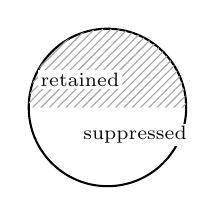
\begin{tikzpicture}[voliphys]
  \draw[volishell] (0,0) circle (1.0);
  \fill[pattern=north east lines, pattern color=black!35] (0,0) -- (1,0) arc (0:180:1) -- cycle;
  \node[volilabel, font=\scriptsize] at (-0.35,0.35) {retained};
  \node[volilabel, font=\scriptsize] at (0.35,-0.35) {suppressed};
\end{tikzpicture}%
}

% --- Lorentz reciprocity: two field configurations ---
\newcommand{\VolIPhysLorentzReciprocity}{%
\begin{tikzpicture}[voliphys]
  \draw[volisrc] (-1.4,0.5) circle (2pt);
  \draw[volisrc] (1.4,0.5) circle (2pt);
  \draw[volifield] (-1.1,0.5) .. controls (0,1.1) .. (1.1,0.5);
  \draw[volisrc] (-1.4,-0.5) circle (2pt);
  \draw[volisrc] (1.4,-0.5) circle (2pt);
  \draw[volifield, dashed] (-1.1,-0.5) .. controls (0,-1.1) .. (1.1,-0.5);
  \node[volilabel, font=\scriptsize] at (0,0) {swap $(1,2)$};
\end{tikzpicture}%
}

% --- Spectral propagating vs evanescent ---
\newcommand{\VolIPhysSpectralRadiationCriterion}{%
\begin{tikzpicture}[voliphys]
  \draw[voliaxis] (-2,0) -- (2,0) node[right,font=\scriptsize] {$k_r$};
  \draw[volipoynt] (0.3,0) -- (0.3,0.8);
  \draw[volipoynt] (0.9,0) -- (0.9,0.55);
  \draw[volifield, dashed] (1.5,0) -- (1.5,0.35);
  \node[volilabel, font=\scriptsize] at (-1.2,0.55) {propagating};
  \node[volilabel, font=\scriptsize] at (1.5,0.55) {evanescent};
\end{tikzpicture}%
}

% --- First-order curl coupling in $\mathcal{M}_\omega$ (Fig. 2.4) ---
\newcommand{\VolIPhysFirstOrderCurlCoupling}{%
\begin{tikzpicture}[voliphys]
  \draw[volishell, fill=black!3] (-1.05,-0.7) rectangle (1.05,0.7);
  \draw[volifield] (-0.55,0.2) -- (0.35,0.4) node[right,font=\scriptsize] {$\E$};
  \draw[volipoynt] (0.25,-0.3) -- (0.95,-0.55) node[right,font=\scriptsize] {$\H$};
  \draw[voliaxis, gray!50!black] (0.55,0.5) arc (130:20:0.38);
  \node[volilabel, font=\scriptsize, gray!50!black] at (0.75,0.62) {$\curl\E$};
  \draw[voliaxis, gray!45!black] (0.45,-0.62) arc (-20:-160:0.38);
  \node[volilabel, font=\scriptsize, gray!45!black] at (0.65,-0.72) {$\curl\H$};
  \draw[volisrc] (-0.9,0) circle (2pt);
  \node[volilabel, font=\scriptsize] at (-0.9,-0.35) {$\Jimp$};
\end{tikzpicture}%
}

% --- Outgoing selector: evanescent decay vs outgoing radiation (Fig. 2.x) ---
\newcommand{\VolIPhysOutgoingSelector}{%
\begin{tikzpicture}[voliphys]
  \draw[volishell, fill=black!4] (-0.28,-0.18) rectangle (0.28,0.18);
  \draw[volishelld] (0,0) circle (0.85);
  \node[volilabel, font=\scriptsize] at (-0.65,0.65) {full $(\E,\H)$};
  \draw[volifield, dashed] (0.32,0.05) .. controls (0.7,0.35) .. (1.05,0.2);
  \node[volilabel, font=\scriptsize] at (0.85,0.5) {$\Pi_{\mathrm{ev}}$};
  \draw[volipoynt] (0.88,0) -- (1.55,0.02) node[midway,above,font=\scriptsize] {$\mathcal{O}_{\mathrm{out}}$};
  \draw[volishell] (2.05,0) circle (0.5);
  \foreach \a in {40,130,220,310} {\draw[volipoynt] (2.05,0) ++(\a:0.28) -- ++(\a:0.17);}
  \node[volilabel] at (2.05,-0.75) {$\mathcal{F}_{\mathrm{rad}}$};
\end{tikzpicture}%
}

% --- Modal bilinear coupling through radiation eigenmodes ---
\newcommand{\VolIPhysModalCoupling}{%
\begin{tikzpicture}[voliphys]
  \draw[volisrc] (-1.45,0.45) circle (2pt);
  \draw[volisrc] (-1.45,-0.45) circle (2pt);
  \node[volilabel, font=\scriptsize] at (-1.45,-0.85) {$\Jimp^{(1)},\Jimp^{(2)}$};
  \draw[volishell] (0.55,0) circle (0.9);
  \foreach \a in {0,45,...,315} {
    \pgfmathsetmacro{\len}{0.3+0.28*sin(\a)}
    \draw[volipoynt] (0.55,0) ++(\a:0.22) -- ++(\a:{\len*0.55});
  }
  \node[volilabel] at (0.55,1.15) {$\mathbf{u}_n$};
  \draw[volifield] (-1.15,0.35) .. controls (-0.25,0.55) .. (0.1,0.25);
  \draw[volifield, dashed] (-1.15,-0.35) .. controls (-0.25,-0.55) .. (0.1,-0.25);
  \node[volilabel, font=\scriptsize] at (1.75,0) {$\mathfrak{C}_\omega$};
\end{tikzpicture}%
}

% --- Ch.1: reactive near zone vs radiative shell (Fig. 1.1) ---
\newcommand{\VolIPhysReactiveVsRadiative}{%
\begin{tikzpicture}[voliphys]
  \draw[volishelld, fill=black!4] (-0.35,-0.35) rectangle (0.35,0.35);
  \draw[volisrc] (0,0) circle (1.5pt);
  \node[volilabel, font=\scriptsize] at (0,-0.62) {bounded source};
  \draw[volishelld] (0,0) circle (0.58);
  \foreach \a in {20,80,140,200,260,320} {
    \draw[gray!40!black, -{Latex[length=1.6mm,width=1mm]}, line width=0.55pt]
      ({0.42*cos(\a)},{0.42*sin(\a)}) arc [start angle=\a, end angle=\a+50, radius=0.42];
  }
  \node[volilabel, font=\scriptsize, align=center] at (-1.55,0.45) {reactive\\$\mathbf{P}$};
  \draw[volishell] (0,0) circle (1.38);
  \node[volilabel, font=\scriptsize] at (1.72,0.05) {$\Gamma_R$};
  \foreach \a in {0,45,90,135,180,225,270,315} {
    \draw[volipoynt] ({1.38*cos(\a)},{1.38*sin(\a)}) -- ({1.78*cos(\a)},{1.78*sin(\a)});
  }
  \node[volilabel, font=\scriptsize, align=center] at (0,2.0)
    {$\oint_{\Gamma_R}\Re\{\mathbf{S}_\mathrm{c}\!\cdot\!\hat{\mathbf{n}}\}\,dS$};
\end{tikzpicture}%
}

% --- Ch.1: Gaussian waist and finite analysis domain ---
\newcommand{\VolIPhysGaussianWaist}{%
\begin{tikzpicture}[voliphys]
  \draw[voliaxis] (-2,0) -- (2,0) node[right, font=\scriptsize] {$x$};
  \draw[volifield, line width=0.75pt] plot[domain=-2:2,samples=60] (\x,{0.85*exp(-\x*\x/0.8)});
  \node[volilabel, font=\scriptsize] at (0,1.05) {$\exp(-r^2/w_0^2)$};
  \draw[volishelld] (-1.55,-0.45) rectangle (1.55,1.15);
  \node[volilabel, font=\scriptsize] at (-1.55,-0.65) {$[-10w_0,10w_0]^3$};
  \draw[volishelld, gray!45!black] (-0.5,-0.45) rectangle (0.5,1.15);
  \node[volilabel, font=\scriptsize] at (0.5,-0.65) {$[-w_0,w_0]^3$};
  \draw[volishell] (0,-0.12) circle (0.95);
  \node[volilabel, font=\scriptsize] at (1.35,-0.12) {$S$};
\end{tikzpicture}%
}

% --- Ch.1: azimuthal filament loop (dipole radiator) ---
\newcommand{\VolIPhysDipoleLoop}{%
\begin{tikzpicture}[voliphys]
  \draw[volishell, line width=0.85pt] (0,0) circle (0.85);
  \draw[gray!40!black, -{Latex[length=2mm,width=1.3mm]}, thick]
    (0.85,0) arc [start angle=0, end angle=300, radius=0.85];
  \node[volilabel, font=\scriptsize] at (60:1.05) {$I_0\hat{\boldsymbol{\phi}}$};
  \node[volilabel, font=\scriptsize] at (0,-1.05) {$b=3\,\mathrm{cm}$};
  \draw[volishelld] (0,0) circle (1.04);
  \node[volilabel, font=\scriptsize] at (45:1.55) {$kr=6.3$};
  \draw[volishelld, dotted] (0,0) circle (0.5);
  \node[volilabel, font=\scriptsize] at (225:0.58) {$kr=0.63$};
\end{tikzpicture}%
}

% --- Ch.1: TE$_{10}$ rectangular waveguide cross-section ---
\expandafter\newcommand\csname VolIPhysWaveguideTE10\endcsname{%
\begin{tikzpicture}[voliphys]
  \draw[volishell, line width=0.85pt] (-1.15,-0.65) rectangle (1.15,0.65);
  \draw[volifield, line width=0.75pt] plot[domain=-1.05:1.05,samples=40]
    (-1.05+2.1*\x/2.1,{0.5*sin(180*\x/2.1)});
  \node[volilabel, font=\scriptsize] at (0,0.82) {TE$_{10}$};
  \draw[volifield] (-1.45,0) -- (-1.15,0);
  \node[volilabel, font=\scriptsize] at (-1.55,0) {$\Jimp$};
  \node[volilabel, font=\scriptsize] at (0,-0.92) {$a\times b$, PEC};
\end{tikzpicture}%
}

% --- Ch.1: torque balance on spherical control shell ---
\newcommand{\VolIPhysTorqueBalanceSurface}{%
\begin{tikzpicture}[voliphys]
  \draw[volishell] (0,0) circle (0.86);
  \node[volilabel] at (1.2,0) {$S_R$};
  \draw[voliaxis] (0,-0.2) -- (0,1.55) node[above, font=\scriptsize] {$\hat{\mathbf{z}}$};
  \draw[volipoynt] (0.85,0) -- (1.15,0) node[above, font=\scriptsize] {$\hat{\mathbf{n}}$};
  \foreach \a in {30,90,150,210,270,330} {
    \draw[volifield, opacity=0.55] (\a:0.55) -- (\a:0.78);
  }
  \node[volilabel, font=\scriptsize] at (0,-1.45) {$m{=}0$ vs.\ $m{\neq}0$};
\end{tikzpicture}%
}

% --- Ch.1: physical rotation vs phased feed on $S_R$ ---
\newcommand{\VolIPhysRotationDuality}{%
\begin{tikzpicture}[voliphys]
  \begin{scope}[shift={(-2.35,0)}]
    \draw[volishell] (0,0) circle (0.55);
    \draw[volipoynt] (0,0) -- (0,0.72) node[left, font=\scriptsize] {$\mathbf{p}$};
    \draw[gray!40!black, -{Latex[length=1.8mm,width=1.2mm]}]
      (0.45,0) arc [start angle=0, end angle=270, radius=0.45];
    \node[volilabel, font=\scriptsize] at (0,-0.78) {(a) rotating source};
  \end{scope}
  \begin{scope}[shift={(2.35,0)}]
    \draw[volisrc] (0,0) circle (2pt);
    \draw[volishelld] (0,0) circle (0.55);
    \foreach \a in {0,45,...,315} {
      \draw[volishelld] (0,0) -- ({0.55*cos(\a)},{0.55*sin(\a)});
    }
    \node[volilabel, font=\scriptsize] at (0,-0.78) {(b) phased feed};
  \end{scope}
  \draw[volishell] (0,0) circle (0.97);
  \node[volilabel, font=\scriptsize] at (1.35,0.2) {$S_R$};
  \draw[volifield, decorate, decoration={snake, amplitude=0.5mm, segment length=2.5mm}]
    (-0.7,0.15) .. controls (0,0.55) .. (0.7,0.15);
\end{tikzpicture}%
}

% --- Ch.1: counter-rotating beams on observation aperture ---
\newcommand{\VolIPhysCounterRotatingAperture}{%
\begin{tikzpicture}[voliphys]
  \draw[volishell] (-1.05,-0.85) rectangle (1.05,0.85);
  \node[volilabel, font=\scriptsize] at (0,1.05) {$S_o$ (open plane)};
  \draw[volifield] (-1.55,0.38) -- (-1.05,0.38);
  \draw[volifield] (-1.55,-0.38) -- (-1.05,-0.38);
  \draw[volipoynt] (-1.35,0.55) arc (90:450:0.18);
  \draw[volipoynt] (-1.35,-0.55) arc (-90:270:0.18);
  \node[volilabel, font=\scriptsize] at (-1.75,0.38) {$+m$};
  \node[volilabel, font=\scriptsize] at (-1.75,-0.38) {$-m$};
  \foreach \a in {45,135,225,315} {
    \draw[black, line width=0.5pt] (0,0) -- (\a:0.65);
  }
  \node[volilabel, font=\scriptsize] at (0,0.55) {$P_+=P_-$};
  \node[volilabel, font=\scriptsize] at (0,-0.55) {$\dot J_z{=}0$};
  \draw[voliaxis] (0,-0.15) -- (0,0.55);
  \node[volilabel, font=\scriptsize] at (0.12,0.62) {$\hat{\mathbf{z}}$};
\end{tikzpicture}%
}

% --- Ch.1 Stage 2.12: three physical consequences of radiation (opening triptych) ---
\newcommand{\VolIPhysThreeRadiationConsequences}{%
\begin{tikzpicture}[voliphys]
  \begin{scope}[shift={(-2.45,0)}]
    \draw[volifield] (-1.0,0) -- (-0.15,0);
    \draw[volishell, volihatch] (-0.1,-0.38) rectangle (0.65,0.38);
    \draw[volipoynt] (0.28,0.38) -- (0.28,0.88);
    \node[volilabel, font=\scriptsize] at (0.28,1.02) {$\langle\mathbf{S}\rangle/c$};
    \node[volilabel, font=\scriptsize, align=center] at (0.28,-0.78) {linear\\momentum};
  \end{scope}
  \begin{scope}[shift={(0,0)}]
    \draw[volifield, decorate, decoration={snake, amplitude=0.35mm, segment length=2mm}] (-1.0,0.12) -- (-0.2,0.12);
    \draw[volishell] (0.05,-0.28) rectangle (0.45,0.28);
    \draw[volishelld] (0.62,-0.32) -- (0.62,0.32);
    \draw[volipoynt] (0.82,0) arc (0:300:0.2);
    \node[volilabel, font=\scriptsize] at (0.25,0.55) {$\sigma{=}{\pm}1$};
    \node[volilabel, font=\scriptsize, align=center] at (0.25,-0.78) {CP\\torque};
  \end{scope}
  \begin{scope}[shift={(2.45,0)}]
    \draw[volifield] (-0.95,0.22) -- (-0.35,0.22);
    \draw[volifield] (-0.95,-0.22) -- (-0.35,-0.22);
    \node[volilabel, font=\scriptsize] at (-0.65,0.38) {$+m$};
    \node[volilabel, font=\scriptsize] at (-0.65,-0.38) {$-m$};
    \draw[volishell] (-0.35,-0.58) rectangle (0.35,0.58);
    \foreach \a in {45,135,225,315} {\draw[black, line width=0.45pt] (0,0) -- (\a:0.42);}
    \node[volilabel, font=\scriptsize] at (0,0.75) {$P_+=P_-$};
    \node[volilabel, font=\scriptsize] at (0,0.55) {$\dot J_z{=}0$};
    \node[volilabel, font=\scriptsize, align=center] at (0,-0.85) {standing\\pattern};
  \end{scope}
\end{tikzpicture}%
}

% --- Ch.1: plane-wave E, H, k, S (handedness) ---
\newcommand{\VolIPhysPlaneWaveHandedness}{%
\begin{tikzpicture}[voliphys]
  \draw[voliaxis] (0,0) -- (2.2,0) node[right, font=\scriptsize] {$\hat{\mathbf{z}}$};
  \draw[-{Latex[length=2mm,width=1.3mm]}, gray!55!black, line width=0.7pt] (0.4,0) -- (0.4,0.85) node[above, font=\scriptsize] {$\E$};
  \draw[-{Latex[length=2mm,width=1.3mm]}, gray!45!black, line width=0.7pt] (1.0,0) -- (1.0,0.85) node[above, font=\scriptsize] {$\H$};
  \draw[volipoynt] (1.55,0) -- (1.55,0.75) node[above, font=\scriptsize] {$\langle\mathbf{S}\rangle$};
  \node[volilabel, font=\scriptsize] at (1.55,-0.35) {$\mathbf{k}$};
\end{tikzpicture}%
}

% --- Ch.1: plane-wave radiation pressure on $V_f$ ($z<0$) ---
\newcommand{\VolIPhysPlaneWaveRadiationPressure}{%
\begin{tikzpicture}[voliphys]
  \draw[volishelld] (-2.15,-0.95) rectangle (2.15,0.95);
  \node[volilabel, font=\scriptsize] at (-1.55,0.75) {$V_f$ ($z<0$)};
  \draw[voliaxis] (-1.9,-0.55) -- (1.9,-0.55) node[right, font=\scriptsize] {$z$};
  \draw[volishell, line width=0.9pt] (-1.85,-0.55) -- (1.85,-0.55);
  \node[volilabel, font=\scriptsize] at (0,-0.72) {$z=0$};
  \draw[volipoynt] (0.15,-0.55) -- (0.15,-0.15) node[right, font=\scriptsize] {$\hat{\mathbf{n}}$};
  \foreach \x in {-1.5,-0.9,-0.3,0.3,0.9,1.5} {
    \draw[volifield] (\x,-0.85) -- (\x,-0.62);
  }
  \node[volilabel, font=\scriptsize] at (-1.65,-0.35) {$\mathbf{k}$};
  \begin{scope}[shift={(-1.05,0.35)}]
    \draw[volishell, volihatch] (-0.32,-0.22) rectangle (0.32,0.22);
    \draw[volipoynt] (0,0.22) -- (0,0.62);
    \node[volilabel, font=\scriptsize, align=center] at (0,-0.42) {absorber\\$p_{\mathrm{abs}}=|\langle\mathbf{S}\rangle|/c$};
  \end{scope}
  \begin{scope}[shift={(1.05,0.35)}]
    \draw[volishell] (-0.32,-0.22) rectangle (0.32,0.22);
    \draw[volifield] (0.32,0.05) .. controls (0.55,0.25) .. (0.32,0.45);
    \draw[volipoynt] (0,0.22) -- (0,0.72);
    \node[volilabel, font=\scriptsize, align=center] at (0,-0.42) {reflector\\$p_{\mathrm{refl}}=2|\langle\mathbf{S}\rangle|/c$};
  \end{scope}
  \draw[volifield] (0.55,0.15) -- (0.55,0.55) node[above, font=\scriptsize] {$\E$};
  \draw[volifield] (0.85,0.15) -- (0.85,0.55) node[above, font=\scriptsize] {$\H$};
\end{tikzpicture}%
}

% --- Ch.1: Green-function source--observation geometry ---
\newcommand{\VolIPhysGreenFunctionGeometry}{%
\begin{tikzpicture}[voliphys]
  \fill[volisrc] (-0.55,0) circle (2pt);
  \node[volilabel, font=\scriptsize] at (-0.55,-0.35) {$\mathbf{r}'$};
  \fill[volisrc] (1.35,0.45) circle (2pt);
  \node[volilabel, font=\scriptsize] at (1.35,0.75) {$\mathbf{r}$};
  \draw[volishelld] (-0.55,0) -- (1.35,0.45);
  \node[volilabel, font=\scriptsize] at (0.35,0.35) {$R$};
  \draw[volipoynt] (1.35,0.45) -- (2.05,0.68);
  \node[volilabel, font=\scriptsize] at (2.15,0.82) {$\hat{\mathbf{r}}$};
  \node[volilabel, font=\scriptsize, align=center] at (0.35,-0.85)
    {$e^{-\jj k_0 R}/(4\pi R)$};
  \draw[volishelld] (1.35,0.45) circle (0.55);
  \node[volilabel, font=\scriptsize] at (2.05,0.15) {far zone};
\end{tikzpicture}%
}

% --- Ch.1: Beth experiment schematic ---
\newcommand{\VolIPhysBethSchematic}{%
\begin{tikzpicture}[voliphys]
  \draw[volifield, decorate, decoration={snake, amplitude=0.4mm, segment length=2mm}] (-2.15,0.2) -- (-0.6,0.2);
  \draw[-{Latex[length=1.6mm,width=1mm]}, gray!50!black, line width=0.55pt]
    (-1.35,0.45) arc (120:420:0.2);
  \node[volilabel, font=\scriptsize] at (-1.35,0.75) {CP ($\sigma{=}+1$)};
  \draw[volishell, volihatch] (-0.48,-0.38) rectangle (0.48,0.38);
  \node[volilabel, font=\scriptsize] at (0,-0.62) {birefringent plate};
  \draw[volishelld, line width=0.55pt] (0.58,0) -- (0.58,1.35);
  \draw[volishell, line width=0.65pt] (0.38,1.35) rectangle (0.78,1.52);
  \node[volilabel, font=\scriptsize, align=center] at (0.58,-0.95) {torsion wire};
  \draw[-{Latex[length=1.8mm,width=1.1mm]}, gray!45!black, line width=0.6pt]
    (0,0.38) arc (85:395:0.24);
  \node[volilabel, font=\scriptsize] at (0.38,0.78) {$\boldsymbol{\tau}_{\mathrm{load}}$};
\end{tikzpicture}%
}

% --- Ch.1: dipole three-zone radii ---
\newcommand{\VolIPhysDipoleThreeZones}{%
\begin{tikzpicture}[voliphys]
  \draw[voliaxis, line width=0.55pt] (0,-0.2) -- (0,1.05);
  \node[volilabel, font=\scriptsize] at (0.12,1.12) {$\hat{\mathbf{z}}$};
  \fill[volisrc] (0,0) circle (2.5pt);
  \draw[volishell, line width=0.65pt] (0,0) -- (0,0.42);
  \node[volilabel, font=\scriptsize] at (0.18,0.22) {$\mathbf{p}$};
  \draw[volishelld] (0,0) circle (0.45);
  \node[volilabel, font=\scriptsize] at (-0.72,0.42) {$kr{=}0.5$};
  \node[volilabel, font=\scriptsize, align=center] at (-1.15,0.05) {near\\$r^{-3}$};
  \draw[volishell, line width=0.65pt] (0,0) circle (0.82);
  \node[volilabel, font=\scriptsize] at (0.62,0.72) {$kr{\sim}1$};
  \node[volilabel, font=\scriptsize, align=center] at (0,1.25) {transition\\$r^{-2}$};
  \draw[volishell, line width=0.75pt] (0,0) circle (1.32);
  \node[volilabel, font=\scriptsize] at (1.0,-0.42) {$kr{=}10$};
  \node[volilabel, font=\scriptsize, align=center] at (1.15,0.35) {far\\$r^{-1}$};
  \foreach \a in {0,45,90,135,180,225,270,315} {
    \draw[volipoynt] (\a:1.05) -- (\a:1.28);
  }
\end{tikzpicture}%
}

% --- Ch.1: open observation plane vs closed enclosing sphere ---
\newcommand{\VolIPhysOpenPlaneVsClosedSphere}{%
\begin{tikzpicture}[voliphys]
  \draw[volisrc] (0,0) circle (2pt);
  \node[volilabel, font=\scriptsize] at (0,-0.35) {source};
  \draw[volishell, fill=black!3] (-0.05,-1.05) -- (0.05,-1.05) -- (0.05,1.05) -- (-0.05,1.05) -- cycle;
  \node[volilabel, font=\scriptsize] at (0.55,0) {$S_o$ (open)};
  \draw[volifield] (-1.2,0.35) -- (-0.05,0.35);
  \draw[volifield] (-1.2,-0.35) -- (-0.05,-0.35);
  \draw[volishell] (0,0) circle (1.25);
  \node[volilabel, font=\scriptsize] at (0.9,0.9) {$\Gamma_R$ (closed)};
  \foreach \a in {30,120,210,300} {\draw[volipoynt] (\a:0.95) -- (\a:1.15);}
\end{tikzpicture}%
}

% --- Ch.2: causal light cone ---
\newcommand{\VolIPhysCausalLightCone}{%
\begin{tikzpicture}[voliphys]
  \draw[volisrc] (0,0) circle (2pt);
  \node[volilabel, font=\scriptsize] at (0,-0.35) {source event};
  \draw[volishelld] (0,0) -- (1.8,1.8);
  \draw[volishelld] (0,0) -- (1.8,-1.8);
  \draw[volipoynt, dashed] (0,0) -- (1.5,0);
  \node[volilabel, font=\scriptsize] at (1.65,0.15) {$c_0 t$};
  \node[volilabel, font=\scriptsize] at (1.0,1.05) {retarded cone};
\end{tikzpicture}%
}

% --- Ch.2: Sommerfeld far zone on sphere ---
\newcommand{\VolIPhysSommerfeldFarZone}{%
\begin{tikzpicture}[voliphys]
  \draw[volisrc] (0,0) circle (2pt);
  \draw[volishelld] (0,0) circle (0.55);
  \draw[volishell] (0,0) circle (1.35);
  \foreach \a in {0,30,...,330} {
    \draw[volipoynt] (\a:0.95) -- (\a:1.25);
  }
  \node[volilabel, font=\scriptsize] at (0,1.55) {$r\to\infty$};
  \node[volilabel, font=\scriptsize] at (0,-1.55) {$e^{-\jj k_0 r}/r$};
\end{tikzpicture}%
}

% --- Ch.2: volume / surface / Huygens integral routes ---
\newcommand{\VolIPhysIntegralRoutes}{%
\begin{tikzpicture}[voliphys]
  \draw[volishell, fill=black!4] (-0.35,-0.25) rectangle (0.35,0.25);
  \node[volilabel, font=\scriptsize] at (0,-0.55) {$\Jimp$ in $V$};
  \draw[volishell] (1.35,0) circle (0.55);
  \node[volilabel, font=\scriptsize] at (1.35,-0.85) {$\Gamma$};
  \draw[volifield] (0.4,0.05) .. controls (0.8,0.35) .. (1.0,0.15);
  \draw[volifield, dashed] (0.35,0) -- (0.8,0);
  \node[volilabel, font=\scriptsize] at (0.55,0.45) {volume};
  \node[volilabel, font=\scriptsize] at (0.55,-0.25) {Huygens};
\end{tikzpicture}%
}

% --- Ch.2: spectral decomposition on sphere ---
\newcommand{\VolIPhysSpectralDecomposition}{%
\begin{tikzpicture}[voliphys]
  \draw[volishell] (0,0) circle (1.0);
  \foreach \a in {0,40,...,320} {
    \pgfmathsetmacro{\len}{0.35+0.4*sin(\a)}
    \draw[volipoynt] (\a:0.2) -- (\a:{\len});
  }
  \node[volilabel, font=\scriptsize] at (0,-1.35) {$\tilde{\E}(\mathbf{k})$ on $S^2$};
\end{tikzpicture}%
}

% --- Ch.2: rotation of angular spectrum ---
\newcommand{\VolIPhysRotationCovariance}{%
\begin{tikzpicture}[voliphys]
  \begin{scope}
    \draw[volishell] (0,0) circle (0.75);
    \draw[volifield] (-0.5,0) -- (0.5,0.2);
    \node[volilabel, font=\scriptsize] at (0,-1.05) {$\mathfrak{F}$};
  \end{scope}
  \node at (1.55,0) {$\rho(g)$};
  \begin{scope}[shift={(2.8,0)}]
    \draw[volishell] (0,0) circle (0.75);
    \draw[volifield] (-0.35,0.35) -- (0.45,0.05);
    \node[volilabel, font=\scriptsize] at (0,-1.05) {$\rho(g)\mathfrak{F}$};
  \end{scope}
\end{tikzpicture}%
}

% --- Ch.2: non-radiating loop cancellation ---
\newcommand{\VolIPhysNRCurrentConfigs}{%
\begin{tikzpicture}[voliphys]
  \draw[volishell] (0,0) circle (0.65);
  \draw[gray!40!black, thick, -{Latex[length=1.8mm]}] (0.65,0) arc (0:180:0.65);
  \draw[gray!40!black, thick, -{Latex[length=1.8mm]}] (-0.65,0) arc (180:360:0.65);
  \draw[volishelld] (0,0) circle (1.35);
  \node[volilabel, font=\scriptsize] at (0,-1.55) {cancelled far field};
\end{tikzpicture}%
}

% --- Ch.3: operator / state / chart distinction (physical panels) ---
\newcommand{\VolIPhysThreeLevelDistinction}{%
\begin{tikzpicture}[voliphys]
  \begin{scope}[shift={(-2.4,0)}]
    \draw[volishell, fill=black!4] (-0.3,-0.2) rectangle (0.3,0.2);
    \draw[volishell] (0,0) circle (0.75);
    \node[volilabel, font=\scriptsize] at (0,-1.05) {$\mathcal{R}_\omega[\Jimp]$};
  \end{scope}
  \begin{scope}
    \draw[volishell] (0,0) circle (0.75);
    \foreach \a in {0,60,...,300} {\draw[volipoynt] (\a:0.35) -- (\a:0.6);}
    \node[volilabel, font=\scriptsize] at (0,-1.05) {$\{c_\alpha\}$};
  \end{scope}
  \begin{scope}[shift={(2.4,0)}]
    \draw[volishell] (0,0) circle (0.75);
    \draw[volipoynt] (0.75,0) -- (1.05,0);
    \node[volilabel, font=\scriptsize] at (0,-1.05) {flux on $\Gamma_R$};
  \end{scope}
\end{tikzpicture}%
}

% --- Ch.3: reciprocity inner product on sphere ---
\newcommand{\VolIPhysReciprocityInnerProduct}{%
\begin{tikzpicture}[voliphys]
  \draw[volishell] (0,0) circle (1.0);
  \draw[volifield] (-0.8,0.3) .. controls (0,0.8) .. (0.8,0.3);
  \draw[volifield, dashed] (-0.8,-0.3) .. controls (0,-0.8) .. (0.8,-0.3);
  \node[volilabel, font=\scriptsize] at (0,0) {$\langle\cdot,\cdot\rangle_{\mathrm{rad}}$};
\end{tikzpicture}%
}

% --- Ch.3: continuous vs discrete spectrum ---
\newcommand{\VolIPhysContinuousDiscreteSpectral}{%
\begin{tikzpicture}[voliphys]
  \draw[voliaxis] (-2,0) -- (2,0);
  \draw[volifield] plot[domain=-1.8:1.8,samples=40] (\x,{0.35*exp(-\x*\x/1.2)});
  \foreach \x in {-1.2,-0.4,0.4,1.2} {
    \draw[volipoynt] (\x,0) -- (\x,{0.35*exp(-\x*\x/1.2)});
  }
  \node[volilabel, font=\scriptsize] at (-1.4,0.55) {continuous};
  \node[volilabel, font=\scriptsize] at (1.2,0.55) {discrete};
\end{tikzpicture}%
}

% --- Ch.3: nested radiative domains (Gelfand-style) ---
\newcommand{\VolIPhysGelfandTripleRadiative}{%
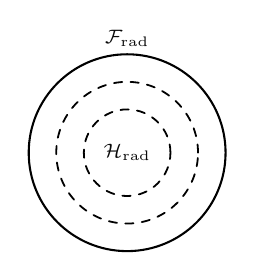
\begin{tikzpicture}[voliphys]
  \draw[volishelld] (0,0) circle (0.55);
  \draw[volishelld] (0,0) circle (0.9);
  \draw[volishell] (0,0) circle (1.25);
  \node[volilabel, font=\scriptsize] at (0,0) {$\mathcal{H}_{\mathrm{rad}}$};
  \node[volilabel, font=\scriptsize] at (0,1.45) {$\mathcal{F}_{\mathrm{rad}}$};
\end{tikzpicture}%
}

% --- Ch.3: orbital and spin on sphere ---
\newcommand{\VolIPhysOrbitalSpinSplit}{%
\begin{tikzpicture}[voliphys]
  \draw[volishell] (0,0) circle (0.9);
  \draw[voliaxis] (0,-0.15) -- (0,1.25) node[above, font=\scriptsize] {$\mathbf{J}_z$};
  \draw[gray!40!black, -{Latex[length=1.6mm]}] (0.7,0) arc (0:300:0.7);
  \node[volilabel, font=\scriptsize] at (0.95,0.35) {$\mathbf{L}$};
  \node[volilabel, font=\scriptsize] at (-0.95,-0.35) {$\mathbf{S}$};
\end{tikzpicture}%
}

% --- Ch.3: SO(3) irrep as angular sector ---
\expandafter\newcommand\csname VolIPhysSO3IrrepBlock\endcsname{%
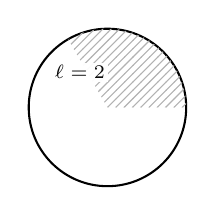
\begin{tikzpicture}[voliphys]
  \draw[volishell] (0,0) circle (1.0);
  \fill[pattern=north east lines, pattern color=black!30] (0,0) -- (1,0) arc (0:120:1) -- cycle;
  \node[volilabel, font=\scriptsize] at (-0.35,0.45) {$\ell=2$};
\end{tikzpicture}%
}

% --- Ch.3: Wigner rotation of sphere ---
\newcommand{\VolIPhysWignerRotation}{%
\begin{tikzpicture}[voliphys]
  \draw[volishell] (0,0) circle (0.85);
  \draw[voliaxis] (0,0) -- (0,1.05);
  \draw[gray!40!black, -{Latex[length=1.8mm]}] (0.55,0) arc (0:270:0.55);
  \node[volilabel, font=\scriptsize] at (0,-1.15) {$D^{(\ell)}_{mm'}(g)$};
\end{tikzpicture}%
}

% --- Ch.3: helicity / polarization on sphere ---
\newcommand{\VolIPhysHelicityPolarizationSplit}{%
\begin{tikzpicture}[voliphys]
  \draw[volishell] (0,0) circle (0.9);
  \draw[volifield] (-0.6,0) .. controls (0,0.55) .. (0.6,0);
  \draw[volipoynt, dashed] (-0.6,0) .. controls (0,-0.55) .. (0.6,0);
  \node[volilabel, font=\scriptsize] at (0,-1.15) {$\sigma=\pm1$};
\end{tikzpicture}%
}

% --- Ch.3: radial outgoing gate ---
\newcommand{\VolIPhysRadialOutgoingGate}{%
\begin{tikzpicture}[voliphys]
  \draw[volisrc] (0,0) circle (2pt);
  \draw[volishelld] (0,0) circle (0.45);
  \draw[volishell] (0,0) circle (1.05);
  \draw[volipoynt] (0.45,0) -- (1.05,0);
  \node[volilabel, font=\scriptsize] at (0.75,0.25) {$h_n^{(1)}$};
\end{tikzpicture}%
}

% --- Ch.3: Debye poloidal/toroidal circulation ---
\newcommand{\VolIPhysDebyeCirculation}{%
\begin{tikzpicture}[voliphys]
  \draw[volishell] (0,0) circle (0.95);
  \draw[gray!40!black, -{Latex[length=1.6mm]}] (0.95,0) arc (0:330:0.95);
  \draw[volifield, dashed] (-0.95,0) arc (180:510:0.95);
  \node[volilabel, font=\scriptsize] at (0,-1.25) {poloidal / toroidal};
\end{tikzpicture}%
}

% --- Ch.3: dipole and quadrupole patterns ---
\newcommand{\VolIPhysDipoleQuadrupole}{%
\begin{tikzpicture}[voliphys]
  \begin{scope}[shift={(-1.35,0)}]
    \draw[volisrc] (0,0) circle (2pt);
    \draw[volipoynt] (0,0) -- (0,0.75);
    \draw[volipoynt] (0,0) -- (0,-0.75);
    \node[volilabel, font=\scriptsize] at (0,-1.05) {$\ell=1$};
  \end{scope}
  \begin{scope}[shift={(1.35,0)}]
    \draw[volisrc] (0,0) circle (2pt);
    \draw[volipoynt] (0,0.55) -- (0.45,0.55);
    \draw[volipoynt] (0,-0.55) -- (0.45,-0.55);
    \draw[volipoynt] (0,0.55) -- (-0.45,0.55);
    \draw[volipoynt] (0,-0.55) -- (-0.45,-0.55);
    \node[volilabel, font=\scriptsize] at (0,-1.05) {$\ell=2$};
  \end{scope}
\end{tikzpicture}%
}

% --- Ch.3: half-space image mixing ---
\newcommand{\VolIPhysHalfSpaceMixing}{%
\begin{tikzpicture}[voliphys]
  \draw[volishell, line width=0.9pt] (-1.5,0) -- (1.5,0);
  \node[volilabel, font=\scriptsize] at (1.65,0) {PEC};
  \draw[volisrc] (0,0.55) circle (2pt);
  \draw[volishelld] (0,-0.55) circle (1.5pt);
  \draw[volishell] (1.35,0.85) circle (0.55);
  \draw[volipoynt] (0.55,0.55) .. controls (0.9,0.85) .. (1.1,0.75);
\end{tikzpicture}%
}

% --- Ch.4: realizability spine (geometry to spectrum) ---
\newcommand{\VolIPhysRealizabilitySpine}{%
\begin{tikzpicture}[voliphys]
  \draw[volishell, fill=black!4] (-0.35,-0.25) rectangle (0.35,0.25);
  \node[volilabel, font=\scriptsize] at (0,-0.55) {$\Omega_s$};
  \draw[volishell] (1.55,0) circle (0.75);
  \foreach \a in {20,60,100,140,200,240,280,320} {
    \pgfmathsetmacro{\len}{0.25+0.35*(1-(\a/360))}
    \draw[volipoynt, opacity={0.3+0.5*(1-\a/360)}] (1.55,0) ++(\a:0.25) -- ++(\a:{\len});
  }
  \node[volilabel, font=\scriptsize] at (1.55,1.05) {$\Gamma_R$};
  \node[volilabel, font=\scriptsize] at (1.55,-1.05) {$\sigma_n\downarrow$};
  \draw[volifield] (0.4,0) .. controls (0.8,0.15) .. (1.0,0.05);
\end{tikzpicture}%
}

% --- Ch.4: realizable source manifold on sphere ---
\newcommand{\VolIPhysRealizableManifold}{%
\begin{tikzpicture}[voliphys]
  \draw[volishell, fill=black!4] (-0.3,-0.2) rectangle (0.3,0.2);
  \draw[volishell] (1.4,0) circle (0.85);
  \fill[pattern=north east lines, pattern color=black!25] (1.4,0) -- (2.25,0) arc (0:180:0.85) -- cycle;
  \node[volilabel, font=\scriptsize] at (1.65,0.45) {$\mathcal{S}_{\mathrm{real}}$};
\end{tikzpicture}%
}

% --- Ch.4: PEC slot tangential field ---
\newcommand{\VolIPhysPECSlotTangential}{%
\begin{tikzpicture}[voliphys]
  \draw[volishell, line width=0.9pt] (-1.4,0) -- (1.4,0);
  \draw[volishell] (-0.15,-0.05) rectangle (0.15,0.05);
  \draw[volifield] (-0.15,0.05) -- (-0.15,0.55);
  \draw[volifield] (0.15,0.05) -- (0.15,0.55);
  \node[volilabel, font=\scriptsize] at (0,-0.45) {slot $\Omega_a$};
\end{tikzpicture}%
}

% --- Ch.4: compact source domain ---
\newcommand{\VolIPhysCompactSourceDomain}{%
\begin{tikzpicture}[voliphys]
  \draw[volishell, fill=black!5] (-0.55,-0.35) rectangle (0.55,0.35);
  \node[volilabel, font=\scriptsize] at (0,0) {$D_s$};
  \draw[volishelld] (0,0) circle (1.15);
  \node[volilabel, font=\scriptsize] at (0,-1.35) {$k_0 D_s$ fixed};
\end{tikzpicture}%
}

% --- Ch.4: support volume scaling ---
\newcommand{\VolIPhysSupportVolumeScaling}{%
\begin{tikzpicture}[voliphys]
  \draw[volishell, fill=black!4] (-0.25,-0.15) rectangle (0.25,0.15);
  \draw[volishell, fill=black!4] (1.0,-0.3) rectangle (1.8,0.3);
  \draw[volishell] (2.55,0) circle (0.65);
  \node[volilabel, font=\scriptsize] at (0.35,-0.55) {small};
  \node[volilabel, font=\scriptsize] at (1.4,-0.55) {large};
\end{tikzpicture}%
}

% --- Ch.4: high-$\ell$ tail suppression ---
\newcommand{\VolIPhysHighEllTail}{%
\begin{tikzpicture}[voliphys]
  \draw[volishell] (0,0) circle (1.0);
  \foreach \a in {0,45,...,315} {
    \pgfmathsetmacro{\len}{0.25+0.5*(1-abs(sin(\a)))}
    \draw[volipoynt] (\a:0.15) -- (\a:{\len});
  }
  \node[volilabel, font=\scriptsize] at (0,-1.35) {high $\ell$ suppressed};
\end{tikzpicture}%
}

% --- Ch.4: finite-support spectral restriction ---
\newcommand{\VolIPhysFiniteSupportRestriction}{%
\begin{tikzpicture}[voliphys]
  \draw[volishell] (0,0) circle (1.0);
  \fill[pattern=north east lines, pattern color=black!30] (0,0) circle (0.55);
  \node[volilabel, font=\scriptsize] at (0,0) {$\mathcal{B}_{\mathrm{fs}}$};
  \draw[volishelld] (0,0) circle (0.85);
  \node[volilabel, font=\scriptsize] at (0,-1.35) {$\cap\,\mathcal{E}_{\mathrm{acc}}^{(N)}$};
\end{tikzpicture}%
}

% --- Ch.4: geometry coupling ---
\newcommand{\VolIPhysGeometryCoupling}{%
\begin{tikzpicture}[voliphys]
  \draw[volishell, fill=black!4] (-0.3,-0.2) rectangle (0.3,0.2);
  \draw[volishell] (1.35,0) circle (0.75);
  \draw[volifield] (0.35,0.05) .. controls (0.75,0.35) .. (0.95,0.15);
  \draw[volifield, dashed] (0.35,-0.05) .. controls (0.75,-0.35) .. (0.95,-0.15);
\end{tikzpicture}%
}

% --- Ch.4: SVD tail compression ---
\newcommand{\VolIPhysCouplingTailCompression}{%
\begin{tikzpicture}[voliphys]
  \draw[voliaxis] (-1.8,0) -- (1.8,0) node[right, font=\scriptsize] {$n$};
  \draw[volipoynt] (-1.5,1.2) -- (-1.5,0);
  \draw[volipoynt] (-0.8,0.55) -- (-0.8,0);
  \draw[volipoynt] (0,0.25) -- (0,0);
  \draw[volipoynt] (0.8,0.08) -- (0.8,0);
  \node[volilabel, font=\scriptsize] at (0,1.35) {$\sigma_n$};
\end{tikzpicture}%
}

% --- Ch.4: effective EM dimension ---
\newcommand{\VolIPhysEffectiveDimension}{%
\begin{tikzpicture}[voliphys]
  \draw[volishell] (0,0) circle (1.0);
  \foreach \n in {1,...,4} {
    \draw[volipoynt] ({90-25*\n}:0.2) -- ({90-25*\n}:{0.35+0.15*\n});
  }
  \draw[volishelld] ({90-25*5}:0.2) -- ({90-25*5}:0.35);
  \node[volilabel, font=\scriptsize] at (0,-1.35) {$d_{\mathrm{eff}}(\varepsilon)$};
\end{tikzpicture}%
}

% --- Ch.4: localization-resolution tradeoff ---
\newcommand{\VolIPhysLocResolutionTradeoff}{%
\begin{tikzpicture}[voliphys]
  \draw[volishell, fill=black!4] (-0.2,-0.15) rectangle (0.2,0.15);
  \draw[volishell] (1.2,0) circle (0.55);
  \draw[volishelld] (1.2,0) circle (0.85);
  \node[volilabel, font=\scriptsize] at (0,-0.55) {support};
  \node[volilabel, font=\scriptsize] at (1.2,-1.15) {angular resolution};
\end{tikzpicture}%
}

% --- Ch.4: LG vs VSH relation ---
\newcommand{\VolIPhysLGVSHRelation}{%
\begin{tikzpicture}[voliphys]
  \begin{scope}
    \draw[volishell] (0,0) circle (0.65);
    \draw[volifield] plot[domain=-0.6:0.6,samples=30] (\x,{0.35*exp(-\x*\x/0.15)});
    \node[volilabel, font=\scriptsize] at (0,-0.95) {LG};
  \end{scope}
  \node at (1.35,0) {$\leftrightarrow$};
  \begin{scope}[shift={(2.2,0)}]
    \draw[volishell] (0,0) circle (0.65);
    \foreach \a in {0,60,...,300} {\draw[volipoynt] (\a:0.25) -- (\a:0.5);}
    \node[volilabel, font=\scriptsize] at (0,-0.95) {VSH};
  \end{scope}
\end{tikzpicture}%
}

% --- Ch.4: triple ceiling ---
\newcommand{\VolIPhysTripleCeiling}{%
\begin{tikzpicture}[voliphys]
  \draw[volishell, fill=black!4] (-0.25,-0.15) rectangle (0.25,0.15);
  \draw[volishell] (1.1,0.55) circle (0.45);
  \draw[volishell] (1.1,-0.55) circle (0.45);
  \draw[volishell] (2.0,0) circle (0.45);
  \node[volilabel, font=\scriptsize] at (0,-0.55) {support};
  \node[volilabel, font=\scriptsize] at (1.1,1.15) {synthesis};
  \node[volilabel, font=\scriptsize] at (2.0,0.65) {recovery};
\end{tikzpicture}%
}

% --- Ch.4: compact range geometry ---
\newcommand{\VolIPhysCompactRangeGeometry}{%
\begin{tikzpicture}[voliphys]
  \draw[volisrc] (-1.2,0) circle (2pt);
  \draw[volishell] (0.8,0) circle (0.75);
  \foreach \a in {30,90,150,210,270,330} {
    \draw[volipoynt] (0.8,0) ++(\a:0.35) -- ++(\a:0.22);
  }
  \node[volilabel, font=\scriptsize] at (-1.2,-0.35) {AUT};
  \node[volilabel, font=\scriptsize] at (0.8,-1.05) {$\Gamma_R$};
\end{tikzpicture}%
}

% --- Ch.4: electrical-size aperture ---
\newcommand{\VolIPhysEllMaxAperture}{%
\begin{tikzpicture}[voliphys]
  \draw[volishell] (0,0) circle (1.0);
  \draw[volishell, fill=black!6] (0,0) circle (0.35);
  \node[volilabel, font=\scriptsize] at (0,0) {$k_0 a$};
  \foreach \a in {0,30,...,330} {
    \pgfmathsetmacro{\len}{0.2+0.45*(1-(\a/360))}
    \draw[volipoynt] (\a:0.35) -- (\a:{\len});
  }
\end{tikzpicture}%
}

% --- Ch.1: Maxwell field to conservation chain (classical monograph style) ---
\newcommand{\VolIPhysMaxwellConservationChain}{%
\begin{tikzpicture}[voliphys]
  \node[volilabel, draw=black!55, rounded corners=2pt, minimum width=1.35cm, minimum height=6mm] (mx) at (0,0) {$(\E,\H)$};
  \node[volilabel, draw=black!55, rounded corners=2pt, minimum width=1.1cm, minimum height=6mm] (s) at (2.0,0) {$\mathbf{S}$};
  \node[volilabel, draw=black!55, rounded corners=2pt, minimum width=1.1cm, minimum height=6mm] (g) at (4.0,0) {$\mathbf{g}_{\mathrm{em}}$};
  \node[volilabel, draw=black!55, rounded corners=2pt, minimum width=0.9cm, minimum height=6mm] (t) at (5.85,0) {$\mathbf{T}$};
  \node[volilabel, draw=black!55, rounded corners=2pt, minimum width=0.9cm, minimum height=6mm] (m) at (7.55,0) {$\mathbf{M}$};
  \node[volilabel, draw=black!55, rounded corners=2pt, minimum width=0.9cm, minimum height=6mm] (j) at (9.25,0) {$\mathbf{j}_{\mathrm{em}}$};
  \draw[volipoynt] (mx.east) -- (s.west);
  \draw[volipoynt] (s.east) -- (g.west);
  \draw[volipoynt] (g.east) -- (t.west);
  \draw[volipoynt] (t.east) -- (m.west);
  \draw[volipoynt] (m.east) -- (j.west);
  \node[volilabel, font=\scriptsize] at (1.0,-0.55) {energy};
  \node[volilabel, font=\scriptsize] at (3.0,-0.55) {momentum};
  \node[volilabel, font=\scriptsize] at (6.7,-0.55) {stress};
  \node[volilabel, font=\scriptsize] at (8.4,-0.55) {torque arm};
\end{tikzpicture}%
}

% --- Ch.1: stress traction on a surface element ---
\newcommand{\VolIPhysStressTraction}{%
\begin{tikzpicture}[voliphys]
  \draw[volishell, volihatch] (-0.55,-0.55) rectangle (0.55,0.55);
  \node[volilabel, font=\scriptsize] at (0,-0.75) {matter in $V_m$};
  \draw[volishell] (-0.95,-0.35) -- (0.95,-0.35) -- (0.55,0.35) -- (-0.55,0.35) -- cycle;
  \draw[-{Latex[length=2mm,width=1.3mm]}, gray!60!black, line width=0.65pt]
    (0,0.35) -- (0,0.95);
  \node[volilabel, font=\scriptsize] at (0.15,1.05) {$\hat{\mathbf{n}}$};
  \draw[-{Latex[length=2mm,width=1.3mm]}, gray!45!black, line width=0.65pt]
    (0,0.35) -- (0.75,0.75);
  \node[volilabel, font=\scriptsize] at (0.95,0.9) {$\mathbf{t}=\langle\mathbf{T}\rangle\!\cdot\!\hat{\mathbf{n}}$};
  \draw[volipoynt] (0.35,0.35) -- (0.95,0.35);
  \node[volilabel, font=\scriptsize] at (1.15,0.35) {$\mathbf{r}$};
  \draw[volipoynt] (0,0) -- (-0.42,0.75);
  \node[volilabel, font=\scriptsize] at (-0.55,0.88) {$\mathbf{r}\times\langle\mathbf{T}\rangle\!\cdot\!\hat{\mathbf{n}}$};
\end{tikzpicture}%
}

% --- Ch.1: momentum density and angular-momentum geometry ---
\newcommand{\VolIPhysMomentumAngularGeometry}{%
\begin{tikzpicture}[voliphys]
  \begin{scope}[shift={(-2.1,0)}]
    \fill[volisrc] (0,0) circle (2pt);
    \node[volilabel, font=\scriptsize] at (-0.2,-0.22) {$O$};
    \fill[volisrc] (1.05,0.35) circle (1.8pt);
    \node[volilabel, font=\scriptsize] at (1.05,0.55) {$\mathbf{r}$};
    \draw[volipoynt] (0,0) -- (1.05,0.35);
    \draw[volipoynt] (1.05,0.35) -- (1.05,0.95);
    \node[volilabel, font=\scriptsize] at (1.22,1.05) {$\langle\mathbf{g}_{\mathrm{em}}\rangle$};
    \draw[volipoynt] (0,0) -- (-0.42,0.82);
    \node[volilabel, font=\scriptsize, align=center] at (-0.55,0.95) {$\langle\mathbf{j}_{\mathrm{em}}\rangle$};
    \node[volilabel, font=\scriptsize, align=center] at (0,-0.85) {volume};
  \end{scope}
  \begin{scope}[shift={(2.0,0)}]
    \draw[volishell] (0,0) circle (1.0);
    \node[volilabel, font=\scriptsize] at (1.25,0) {$\Gamma_R$};
    \draw[volishell, volihatch] (0.55,0.15) -- (0.95,0.35) -- (0.75,0.75) -- (0.35,0.55) -- cycle;
    \draw[volipoynt] (0.65,0.45) -- (0.65,0.95);
    \node[volilabel, font=\scriptsize] at (0.78,1.05) {$\hat{\mathbf{n}}$};
    \draw[volipoynt] (0,0) -- (0.65,0.45);
    \node[volilabel, font=\scriptsize] at (0.32,0.28) {$\mathbf{r}$};
    \draw[volipoynt] (0.65,0.45) -- (1.05,0.72);
    \node[volilabel, font=\scriptsize] at (1.18,0.85) {$\langle\mathbf{T}\rangle\!\cdot\!\hat{\mathbf{n}}$};
    \draw[volipoynt] (0,0) -- (-0.35,0.88);
    \node[volilabel, font=\scriptsize, align=center] at (-0.5,1.0) {$\mathbf{r}\times(\langle\mathbf{T}\rangle\!\cdot\!\hat{\mathbf{n}})$};
    \node[volilabel, font=\scriptsize, align=center] at (0,-0.85) {surface};
  \end{scope}
\end{tikzpicture}%
}

% --- Ch.1: azimuthal phase fronts for several $m$ ---
\newcommand{\VolIPhysAzimuthalPhase}{%
\begin{tikzpicture}[voliphys]
  \begin{scope}[shift={(-2.4,0)}]
    \draw[volishell] (0,0) circle (0.55);
    \draw[volifield] (-0.45,0) -- (0.45,0);
    \node[volilabel, font=\scriptsize] at (0,-0.85) {$m=0$};
  \end{scope}
  \begin{scope}[shift={(-0.8,0)}]
    \draw[volishell] (0,0) circle (0.55);
    \draw[volifield] (0.12,0) -- (0.48,0);
    \node[volilabel, font=\scriptsize] at (0,-0.85) {$m=1$};
  \end{scope}
  \begin{scope}[shift={(0.8,0)}]
    \draw[volishell] (0,0) circle (0.55);
    \draw[volifield] (0.12,0) -- (0.48,0);
    \draw[volifield] (0.09,0.09) -- (0.34,0.34);
    \node[volilabel, font=\scriptsize] at (0,-0.85) {$m=2$};
  \end{scope}
  \begin{scope}[shift={(2.4,0)}]
    \draw[volishell] (0,0) circle (0.55);
    \foreach \a in {0,120,240} {
      \draw[volifield, line width=0.45pt] (\a:0.12) -- (\a:0.48);
    }
    \node[volilabel, font=\scriptsize] at (0,-0.85) {$m=3$};
  \end{scope}
\end{tikzpicture}%
}

% --- Ch.1: signed angular-momentum flux on a sphere ---
\newcommand{\VolIPhysSignedAmFlux}{%
\begin{tikzpicture}[voliphys]
  \draw[volishell] (0,0) circle (1.0);
  \fill[volisrc] (0,0) circle (2pt);
  \draw[-{Latex[length=2mm,width=1.3mm]}, gray!45!black, line width=0.65pt]
    (0.75,0.15) -- (1.15,0.35);
  \node[volilabel, font=\scriptsize] at (1.05,0.55) {$+\boldsymbol{\Psi}_J$};
  \draw[-{Latex[length=2mm,width=1.3mm]}, gray!55!black, line width=0.65pt]
    (-0.75,0.15) -- (-1.15,0.35);
  \node[volilabel, font=\scriptsize] at (-1.05,0.55) {$-\boldsymbol{\Psi}_J$};
  \node[volilabel, font=\scriptsize, align=center] at (0,-1.35)
    {$\mathbf{J}_{\mathrm{rad}}=\int_{4\pi}\boldsymbol{\Psi}_J\,d\Omega$};
\end{tikzpicture}%
}

% --- Ch.1: electric dipole radiation pattern $\sin^2\theta$ (meridional plane) ---
\newcommand{\VolIPhysDipoleRadiationPattern}{%
\begin{tikzpicture}[voliphys]
  \draw[voliaxis, line width=0.55pt] (0,-1.5) -- (0,1.5);
  \node[volilabel, font=\scriptsize] at (0.14,1.58) {$\hat{\mathbf{z}}$};
  \draw[volishell, line width=0.7pt] (0,0) -- (0,0.5);
  \node[volilabel, font=\scriptsize] at (0.24,0.25) {$\mathbf{p}$};
  \fill[volisrc] (0,0) circle (1.8pt);
  \draw[volishell, line width=0.85pt, smooth, samples=181, domain=-180:180]
    plot ({1.2*sin(\x)*sin(\x)*sin(\x)},{1.2*sin(\x)*sin(\x)*cos(\x)});
  \draw[gray!45!black, line width=0.4pt, dashed] (-1.35,0) -- (1.35,0);
  \node[volilabel, font=\scriptsize] at (1.38,0.08) {$\theta$};
  \node[volilabel, font=\scriptsize] at (0.08,-1.22) {$\theta{=}0$};
  \node[volilabel, font=\scriptsize] at (0.08,1.22) {$\theta{=}\pi$};
  \node[volilabel, font=\scriptsize] at (0.95,0.12) {max};
  \node[volilabel, font=\scriptsize] at (-0.95,0.12) {max};
  \node[volilabel, font=\scriptsize, align=center] at (0,-1.78)
    {$U(\theta)\propto\sin^2\theta$};
\end{tikzpicture}%
}

% --- Ch.1: plane wave vs localized finite-energy radiator ---
\newcommand{\VolIPhysPlaneWaveVsSource}{%
\begin{tikzpicture}[voliphys]
  \begin{scope}
    \foreach \y in {-0.5,-0.15,0.2,0.55} {
      \draw[volifield] (-1.1,\y) -- (1.1,\y);
    }
    \node[volilabel, font=\scriptsize, align=center] at (0,-0.95) {infinite\\plane wave};
  \end{scope}
  \begin{scope}[shift={(3.0,0)}]
    \fill[volisrc] (0,0) circle (2pt);
    \draw[volishelld] (0,0) circle (0.55);
    \draw[volishell] (0,0) circle (1.05);
    \foreach \a in {25,70,115,205,250,295} {
      \draw[volipoynt] (\a:0.82) -- (\a:0.98);
    }
    \node[volilabel, font=\scriptsize, align=center] at (0,-0.95) {localized\\radiator};
  \end{scope}
\end{tikzpicture}%
}

% --- Ch.1: radial zones $r^{-3}$, $r^{-2}$, $r^{-1}$ ---
\newcommand{\VolIPhysRadialFieldZones}{%
\begin{tikzpicture}[voliphys]
  \fill[volisrc] (0,0) circle (2.5pt);
  \node[volilabel, font=\scriptsize] at (0,-0.28) {dipole};
  \draw[volishelld] (0,0) circle (0.48);
  \node[volilabel, font=\scriptsize, align=center] at (-1.05,0.35) {reactive\\$r^{-3}$};
  \draw[volishell, line width=0.6pt] (0,0) circle (0.88);
  \node[volilabel, font=\scriptsize, align=center] at (0,1.05) {induction\\$r^{-2}$};
  \draw[volishell] (0,0) circle (1.38);
  \node[volilabel, font=\scriptsize, align=center] at (1.05,-0.35) {radiation\\$r^{-1}$};
  \foreach \a in {15,55,95,135,175,215,255,295,335} {
    \draw[volipoynt] (\a:1.12) -- (\a:1.32);
  }
  \node[volilabel, font=\scriptsize, align=center] at (0,-1.65)
    {$kr\ll1$ \ $\rightarrow$ \ $kr\sim1$ \ $\rightarrow$ \ $kr\gg1$};
\end{tikzpicture}%
}

% --- Ch.1 foundation expansion figures ---
\newcommand{\VolIPhysLongTransDecomp}{%
\begin{tikzpicture}[voliphys]
  \coordinate (O) at (0,0);
  \draw[-{Latex[length=2mm,width=1.2mm]}, gray!60!black, line width=0.55pt] (O) -- (1.4,0);
  \draw[-{Latex[length=2mm,width=1.2mm]}, gray!60!black, line width=0.55pt] (O) -- (0,1.2);
  \node[volilabel, font=\scriptsize] at (1.5,0) {$x$};
  \node[volilabel, font=\scriptsize] at (0,1.35) {$y$};
  \draw[-{Latex[length=2.2mm,width=1.3mm]}, gray!45!black, line width=0.65pt]
    (0.2,0.2) -- (1.05,0.95);
  \node[volilabel, font=\scriptsize] at (0.85,1.05) {$\mathbf{F}$};
  \draw[-{Latex[length=1.8mm,width=1.1mm]}, gray!55!black, line width=0.55pt, dashed]
    (0.2,0.2) -- (0.95,0.35);
  \node[volilabel, font=\scriptsize] at (0.55,0.15) {$\mathbf{F}_L$};
  \draw[-{Latex[length=1.8mm,width=1.1mm]}, gray!35!black, line width=0.55pt]
    (0.2,0.2) -- (0.35,0.95);
  \node[volilabel, font=\scriptsize] at (0.15,0.85) {$\mathbf{F}_T$};
  \node[volilabel, font=\scriptsize, align=center] at (0,-0.55)
    {$\mathbf{F}=\mathbf{F}_L+\mathbf{F}_T$};
\end{tikzpicture}%
}

\newcommand{\VolIPhysEquivalentSurface}{%
\begin{tikzpicture}[voliphys]
  \draw[volishell, fill=black!4] (0,0) circle (0.85);
  \fill[gray!35] (0,0) circle (0.35);
  \node[volilabel, font=\scriptsize] at (0,-0.05) {sources};
  \draw[volishell, line width=0.7pt] (0,0) circle (0.85);
  \node[volilabel, font=\scriptsize] at (0.95,0.55) {$S$};
  \foreach \a in {30,110,190,270} {
    \draw[volipoynt] (0,0) ++(\a:0.85) -- ++(\a:0.25);
  }
  \node[volilabel, font=\scriptsize, align=center] at (0,-1.15)
    {$\mathbf{J}_s^{(e)}=\hat{\mathbf{n}}\times\H$};
\end{tikzpicture}%
}

\newcommand{\VolIPhysAngularSpectrumDisk}{%
\begin{tikzpicture}[voliphys]
  \draw[volishell] (-1.1,-0.9) rectangle (1.1,0.9);
  \node[volilabel, font=\scriptsize] at (0,1.05) {$k_y$};
  \node[volilabel, font=\scriptsize] at (1.25,0) {$k_x$};
  \draw[volishell, fill=black!3] (0,0) circle (0.65);
  \node[volilabel, font=\scriptsize] at (0,0) {$k_\rho<k_0$};
  \node[volilabel, font=\scriptsize, align=center] at (0,-1.25)
    {propagating disk; evanescent exterior};
\end{tikzpicture}%
}

\newcommand{\VolIPhysPropagEvanescentWave}{%
\begin{tikzpicture}[voliphys]
  \draw[volishell] (-1.2,0.7) -- (1.2,0.7);
  \node[volilabel, font=\scriptsize] at (0,0.95) {$z=0$};
  \foreach \x in {-0.8,-0.4,0,0.4,0.8} {
    \draw[volifield] (\x,0.7) -- (\x,1.35);
  }
  \node[volilabel, font=\scriptsize] at (-1.35,1.0) {prop.};
  \draw[volishell, dashed] (1.5,0.7) -- (1.5,-0.9);
  \foreach \z in {0.5,0.1,-0.3,-0.7} {
    \draw[volipoynt] (1.5,\z) -- (1.75,\z);
  }
  \node[volilabel, font=\scriptsize, align=center] at (1.65,-1.05)
    {$e^{-\alpha z}$};
\end{tikzpicture}%
}

\newcommand{\VolIPhysCylindricalBessel}{%
\begin{tikzpicture}[voliphys]
  \draw[-{Latex[length=2mm,width=1.2mm]}, gray!60!black] (0,-0.9) -- (0,1.0);
  \draw[-{Latex[length=2mm,width=1.2mm]}, gray!60!black] (-0.9,0) -- (1.0,0);
  \node[volilabel, font=\scriptsize] at (0,1.15) {$z$};
  \node[volilabel, font=\scriptsize] at (1.1,0) {$\rho$};
  \draw[volishell] (0,0) ellipse (0.95 and 0.35);
  \draw[volifield, domain=0:360,samples=60,smooth]
    plot ({0.55*cos(\x)},{0.2*sin(\x)});
  \node[volilabel, font=\scriptsize, align=center] at (0,-1.15)
    {$J_m(k_\rho\rho)e^{\jj m\phi}$};
\end{tikzpicture}%
}

\newcommand{\VolIPhysPhaseWindingSingularity}{%
\begin{tikzpicture}[voliphys]
  \begin{scope}[shift={(-1.7,0)}]
    \draw[volishell] (0,0) circle (0.38);
    \node[volilabel, font=\scriptsize] at (0,-0.62) {$m=0$};
  \end{scope}
  \begin{scope}[shift={(-0.55,0)}]
    \draw[volishell] (0,0) circle (0.38);
    \foreach \a in {0,60,...,300} {\draw[volipoynt] (\a:0.12) arc (\a:\a+45:0.12);}
    \fill (0,0) circle (1.2pt);
    \node[volilabel, font=\scriptsize] at (0,-0.62) {$m=1$};
  \end{scope}
  \begin{scope}[shift={(0.55,0)}]
    \draw[volishell] (0,0) circle (0.38);
    \foreach \a in {0,60,...,300} {\draw[volipoynt] (\a:0.12) arc (\a+45:\a:0.12);}
    \fill (0,0) circle (1.2pt);
    \node[volilabel, font=\scriptsize] at (0,-0.62) {$m=-1$};
  \end{scope}
  \begin{scope}[shift={(1.7,0)}]
    \draw[volishell] (0,0) circle (0.38);
    \foreach \a in {0,40,...,320} {\draw[volipoynt] (\a:0.1) arc (\a:\a+30:0.1);}
    \fill (0,0) circle (1.2pt);
    \node[volilabel, font=\scriptsize] at (0,-0.62) {$m=2$};
  \end{scope}
\end{tikzpicture}%
}

\newcommand{\VolIPhysEllVsM}{%
\begin{tikzpicture}[voliphys]
  \foreach \x/\lab in {0/$Y_1^0$/,1.2/$Y_1^1$/,2.4/$Y_2^0$/,3.6/$Y_2^2$/} {
    \begin{scope}[shift={(\x,0)}]
      \VolIPhysSphericalMode{20+\x*15}
      \node[volilabel, font=\scriptsize] at (0,-1.25) {\lab};
    \end{scope}
  }
\end{tikzpicture}%
}

\newcommand{\VolIPhysTwoElementArray}{%
\begin{tikzpicture}[voliphys]
  \fill[volisrc] (-0.55,0) circle (2pt);
  \fill[volisrc] (0.55,0) circle (2pt);
  \draw[volishell, <->] (-0.55,-0.35) -- (0.55,-0.35);
  \node[volilabel, font=\scriptsize] at (0,-0.55) {$d$};
  \draw[volipoynt] (-0.55,0) -- (-1.1,0.45);
  \draw[volipoynt] (0.55,0) -- (1.1,0.45);
  \node[volilabel, font=\scriptsize] at (0,0.75) {$\theta$};
\end{tikzpicture}%
}

\newcommand{\VolIPhysScatteringAM}{%
\begin{tikzpicture}[voliphys]
  \draw[volishell, fill=black!4] (0,0) circle (0.35);
  \draw[volipoynt] (-1.2,0) -- (-0.45,0);
  \node[volilabel, font=\scriptsize] at (-0.85,0.2) {inc.};
  \draw[volipoynt] (0.45,0.25) -- (1.1,0.55);
  \draw[volipoynt] (0.45,-0.25) -- (1.1,-0.55);
  \node[volilabel, font=\scriptsize] at (0.85,0.55) {sc.};
  \draw[volishell, dashed] (0,0) circle (0.75);
\end{tikzpicture}%
}

\newcommand{\VolIPhysFiniteSourceKa}{%
\begin{tikzpicture}[voliphys]
  \draw[volishell, fill=black!5] (-0.35,-0.35) rectangle (0.35,0.35);
  \node[volilabel, font=\scriptsize] at (0,0) {$ka$};
  \draw[volipoynt] (0.35,0.15) .. controls (0.9,0.5) .. (1.35,0.15);
  \draw[volipoynt] (0.35,-0.15) .. controls (0.9,-0.5) .. (1.35,-0.15);
  \node[volilabel, font=\scriptsize, align=center] at (0,-0.85)
    {small $ka$: low $\ell$};
\end{tikzpicture}%
}

\newcommand{\VolIPhysChapterOneSynthesis}{%
\begin{tikzpicture}[voliphys]
  \node[volilabel, font=\scriptsize, align=center] at (0,1.0)
    {Maxwell $\rightarrow$ angular structure};
  \draw[volishell] (-1.3,0.3) rectangle (1.3,-0.9);
  \node[volilabel, font=\scriptsize, align=center] at (0,0)
    {stress $\rightarrow$ $e^{\jj m\phi}$ $\rightarrow$ radiation};
  \draw[volipoynt] (0,-0.9) -- (0,-1.25);
  \node[volilabel, font=\scriptsize] at (0,-1.45) {Ch.~2--4};
\end{tikzpicture}%
}

% Wrapper sizing consistent with ChOneFigGeo
\newcommand{\VolIPhysFig}[1]{\ChOneFigGeo{#1}}
\newcommand{\VolIPhysFigWide}[1]{\adjustbox{max width=0.88\linewidth, max height=0.38\textheight, center}{#1}}
